\documentclass[10pt]{article}
\usepackage[a4paper,margin=1.8cm]{geometry}\usepackage{needspace}\usepackage{amsmath,amssymb,graphicx,booktabs,longtable,array,hyperref}
\setlength{\parindent}{0pt}\setlength{\parskip}{3pt}\sloppy
\begin{document}
{\LARGE\bfseries Sixteen worked examples of $C\star L$}\\[2pt]
{\large Reflecting generalized circles in $\mathbb P^3(\mathbb C)$: real, complex and mixed}\\[6pt]
\textbf{Setting.} A generalized circle is $C=[a:b:c:d]\in\mathbb P^3(\mathbb C)$, the curve $a(x^2+y^2)+bx+cy+d=0$; lines have $a=0$. With
\[Q(C)=b^2+c^2-4ad,\qquad \langle C,C'\rangle=bb'+cc'-2(ad'+a'd),\]\[C\star L=C-\frac{2\langle C,L\rangle}{Q(L)}\,L\quad(Q(L)\neq0),\qquad \kappa(C,L)=\frac{\langle C,L\rangle^2}{Q(C)\,Q(L)},\]
everything is bilinear over $\mathbb C$ (no complex conjugates). For a real circle $Q/a^2=4r^2$. A point $p=(x_0,y_0)\in\mathbb C^2$ is the point-circle $\mathrm{pt}(p)=[1:-2x_0:-2y_0:x_0^2+y_0^2]$, with $Q=0$, and $\langle \mathrm{pt}(p),C\rangle=-2\,C(p)$; $\infty=[0:0:0:1]$.

\textbf{Facts used.} (i) $C\star L$ is again a generalized circle, $Q(C\star L)=Q(C)$, and $(C\star L)\star L=C$; real mirrors act as reflection in a line or inversion in a circle. (ii) $C\star L=C-kL$ lies in the pencil of $C$ and $L$; if $k\neq0$, i.e.\ $\langle C,L\rangle\neq0$, then $C\cap(C\star L)=C\cap L$. (iii) The common points of $C$ and $L$ on the Möbius quadric $\{Q=0\}$ are the null vectors of $\mathrm{span}(C,L)^\perp$: two, or one double point when $\kappa=1$ (tangency). (iv) $\kappa$ is symmetric and unchanged by every reflection; for two real lines or for a real crossing it is $\cos^2$ of the angle.

\textbf{Caveats.} $Q(L)=0$ (point-circles, isotropic lines $b^2+c^2=0$): $L$ cannot be a mirror, and $\kappa$ is undefined if either $Q$ vanishes. $\langle C,L\rangle=0$: $C\star L=C$, and fact (ii) gives no information. ``Two points'' counts multiplicity and is about the Möbius quadric: a line ($a=0$) meets another line at $\infty$; concentric circles and isotropic lines can lose finite points, which then sit on the quadric over $\infty$ (Examples 5, 10). ``Real picture'' means we draw only real points, or the real trace $\mathrm{Re}\,C\cap\mathrm{Im}\,C$ of a complex circle, and say so.

\textbf{Verification.} Every number below is computed exactly with SymPy and asserted in \texttt{examples16.py}. That includes: the image, $\kappa$, the common points, involution, invariance of $Q$ and $\kappa$, $C\cap(C\star L)=C\cap L$ when $\langle C,L\rangle\neq0$, incidence of the Möbius points, a floating-point re-check under random complex rescaling, and each example's special claims. Log: \texttt{examples16\_verify\_log.txt} (247 checks, no failures).

\smallskip
{\small\setlength{\tabcolsep}{4pt}\begin{longtable}{r>{\raggedright}p{0.34\textwidth}>{\raggedright}p{0.16\textwidth}c>{\raggedright\arraybackslash}p{0.19\textwidth}}\toprule
\# & example & inputs & $\kappa$ & finite common points\\\midrule\endhead
1 & Fold the unit circle along $x=\tfrac12$ & real & $\frac{1}{4}$ & two real\\
2 & The line that misses: $x=2$ & real input, hidden output & $4$ & conjugate pair\\
3 & Just touching: $x+y=\sqrt2$ & real & $1$ & one double point (real)\\
4 & Orthogonal circles: the mirror that does nothing & real & $0$ & two real\\
5 & Concentric circles meet only at infinity & real & $\frac{25}{16}$ & no finite point\\
6 & Two lines at $60^\circ$ & real & $\frac{1}{4}$ & one finite point (and $\infty$)\\
7 & Invert a line: $x=2$ in the unit circle & real input, hidden output & $4$ & conjugate pair\\
8 & A circle with complex centre: $(x-i)^2+y^2=1$ & complex & $-1$ & two real\\
9 & The circle of imaginary radius $x^2+y^2=-1$ & mixed & $- \frac{1}{4}$ & conjugate pair\\
10 & Isotropic lines: $y=ix$, $y=ix+1$, and $y=2ix$ & complex & $0$ & two complex, not conjugate\\
11 & A point as input: the point-circle at $(1,1)$ & real, degenerate & $\text{undefined } (Q(\cdot)=0)$ & conjugate pair\\
12 & A complex mirror makes a real circle non-real & mixed & $\frac{9}{4}$ & two complex, not conjugate\\
13 & Two mirrors make a rotation of order 2, 3, 4, $\infty$, or a complex angle & real and complex & $4$ & one finite point (and $\infty$)\\
14 & The kei law, checked by hand & real & $\frac{4}{5}$ & two real\\
15 & Tangency with complex coefficients & complex & $1$ & one double point (complex)\\
16 & Find the mirror: swap two disjoint circles & real input, imaginary answer & $\frac{121}{16}$ & conjugate pair\\
\bottomrule\end{longtable}}
\newpage
\needspace{12\baselineskip}\subsection*{Example 1. Fold the unit circle along $x=\tfrac12$}
\textbf{Exercise.} Reflect the unit circle $K$ in the line $L:\;x=\tfrac12$. Find $K\star L$, the common points and $\kappa$.

\smallskip\textbf{Solution.} \textbf{Inputs.} $K=[1:0:0:-1]$, i.e.\ $x^2+y^2=1$; \ $L=[0:1:0:- \frac{1}{2}]$, i.e.\ $x=\tfrac12$. \textbf{Numbers.} $Q(K)=4$, $Q(L)=1$, $\langle K,L\rangle=1$, $\kappa=\frac{1}{4}$. \textbf{Image.} $K\star L=K-\tfrac{2\langle K,L\rangle}{Q(L)}L\sim[1:-2:0:0]$, i.e.\ $x^{2} - 2 x + y^{2}=0$. \textbf{Common points} (finite, of $K$ and $L$): $\left(\frac{1}{2},\ - \frac{\sqrt{3}}{2}\right)$, $\left(\frac{1}{2},\ \frac{\sqrt{3}}{2}\right)$ --- two real. The image is the unit circle translated to centre $(1,0)$, as a fold along $x=\tfrac12$ should give. The real crossing angle $\varphi$ satisfies $\kappa=\cos^2\varphi$: here $\varphi=60^\circ$.

\smallskip\emph{Why it is fun.} For a real secant, $\kappa=\cos^2(\text{crossing angle})$; for our sweep $x=t$, $\kappa=t^2$.
\begin{center}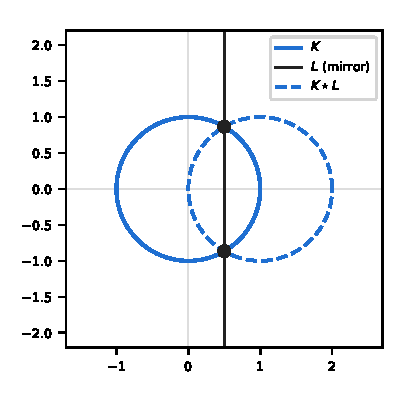
\includegraphics[width=0.31\textwidth]{examples16_figs/ex01.pdf}\\[-2pt]{\footnotesize Real picture: fold along $x=\tfrac12$.}\end{center}

\needspace{12\baselineskip}\subsection*{Example 2. The line that misses: $x=2$}
\textbf{Exercise.} Reflect $K$ in $L:\;x=2$, which misses it. Where do $K$ and $L$ meet?

\smallskip\textbf{Solution.} \textbf{Inputs.} $K=[1:0:0:-1]$, i.e.\ $x^2+y^2=1$; \ $L=[0:1:0:-2]$, i.e.\ $x=2$. \textbf{Numbers.} $Q(K)=4$, $Q(L)=1$, $\langle K,L\rangle=4$, $\kappa=4$. \textbf{Image.} $K\star L=K-\tfrac{2\langle K,L\rangle}{Q(L)}L\sim[1:-8:0:15]$, i.e.\ $x^{2} - 8 x + y^{2} + 15=0$. \textbf{Common points} (finite, of $K$ and $L$): $\left(2,\ - \sqrt{3} i\right)$, $\left(2,\ \sqrt{3} i\right)$ --- conjugate pair. The image $(x-4)^2+y^2=1$ is real, but the common points are the conjugate pair $(2,\pm i\sqrt3)$. The image passes through them too: $4-16+15+(i\sqrt3)^2=0$. In the Short's convention (perpendicular sweep, points at the foot) we draw them as $(2,\pm\sqrt3)$, a point of the hyperbola $t^2-s^2=1$.

\smallskip\emph{Why it is fun.} $\kappa=4>1$: real data, hidden points, and the algebra does not notice.
\begin{center}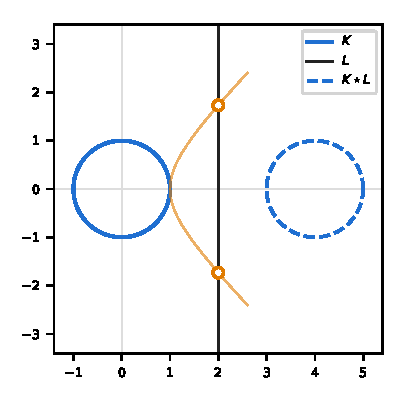
\includegraphics[width=0.31\textwidth]{examples16_figs/ex02.pdf}\\[-2pt]{\footnotesize Real picture; rings: the slice drawing $(2,\pm\sqrt3)$ of the hidden pair $(2,\pm i\sqrt3)$.}\end{center}

\needspace{12\baselineskip}\subsection*{Example 3. Just touching: $x+y=\sqrt2$}
\textbf{Exercise.} Show that $L:\;x+y=\sqrt2$ is tangent to $K$ using only $\kappa$, then find $K\star L$.

\smallskip\textbf{Solution.} \textbf{Inputs.} $K=[1:0:0:-1]$, i.e.\ $x^2+y^2=1$; \ $L=[0:1:1:- \sqrt{2}]$, i.e.\ $x+y=\sqrt2$. \textbf{Numbers.} $Q(K)=4$, $Q(L)=2$, $\langle K,L\rangle=2 \sqrt{2}$, $\kappa=1$. \textbf{Image.} $K\star L=K-\tfrac{2\langle K,L\rangle}{Q(L)}L\sim[1:- 2 \sqrt{2}:- 2 \sqrt{2}:3]$, i.e.\ $x^{2} - 2 \sqrt{2} x + y^{2} - 2 \sqrt{2} y + 3=0$. \textbf{Common points} (finite, of $K$ and $L$): $\left(\frac{\sqrt{2}}{2},\ \frac{\sqrt{2}}{2}\right)$ --- one double point (real). $\kappa=1$, so the two common points merge into one double point. The image circle, centre $(\sqrt2,\sqrt2)$ and radius $1$, touches $K$ at the same point.

\smallskip\emph{Why it is fun.} Tangency is a single equation, $\langle C,L\rangle^2=Q(C)Q(L)$; no square roots are needed.
\begin{center}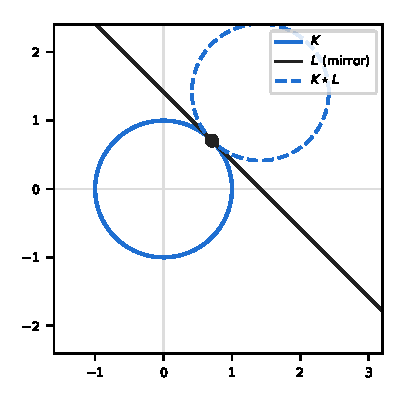
\includegraphics[width=0.31\textwidth]{examples16_figs/ex03.pdf}\\[-2pt]{\footnotesize Real picture: one double point.}\end{center}

\needspace{12\baselineskip}\subsection*{Example 4. Orthogonal circles: the mirror that does nothing}
\textbf{Exercise.} Compute $K\star M$ for $M:\;(x-2)^2+y^2=3$. Do $K$ and $M$ meet?

\smallskip\textbf{Solution.} \textbf{Inputs.} $K=[1:0:0:-1]$, i.e.\ $x^2+y^2=1$; \ $M=[1:-4:0:1]$, i.e.\ $(x-2)^2+y^2=3$. \textbf{Numbers.} $Q(K)=4$, $Q(M)=12$, $\langle K,M\rangle=0$, $\kappa=0$. \textbf{Image.} $K\star M=K-\tfrac{2\langle K,M\rangle}{Q(M)}M\sim[1:0:0:-1]$, i.e.\ $x^{2} + y^{2} - 1=0$. \textbf{Common points} (finite, of $K$ and $M$): $\left(\frac{1}{2},\ - \frac{\sqrt{3}}{2}\right)$, $\left(\frac{1}{2},\ \frac{\sqrt{3}}{2}\right)$ --- two real. $\langle K,M\rangle=0$, so $K\star M=K$ (and $M\star K=M$). They do meet, at $(\tfrac12,\pm\tfrac{\sqrt3}2)$, at right angles ($1+3=2^2$). Here $C\cap(C\star L)=C$, so the image tells us nothing about the common points: this is the one exception to ``$C\star L$ meets $C$ where $L$ does''.

\smallskip\emph{Why it is fun.} $\kappa=0$ means orthogonal. The mirror fixes the circle without fixing its points: inversion in $M$ swaps the two arcs of $K$.
\begin{center}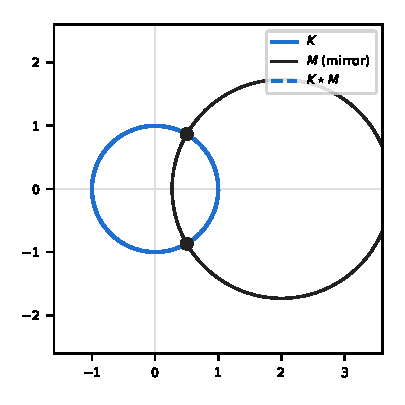
\includegraphics[width=0.31\textwidth]{examples16_figs/ex04.pdf}\\[-2pt]{\footnotesize Real picture: orthogonal circles; the image is $K$ itself.}\end{center}

\needspace{12\baselineskip}\subsection*{Example 5. Concentric circles meet only at infinity}
\textbf{Exercise.} Invert $K$ in $M:\;x^2+y^2=4$. Where do two concentric circles meet?

\smallskip\textbf{Solution.} \textbf{Inputs.} $K=[1:0:0:-1]$, i.e.\ $x^2+y^2=1$; \ $M=[1:0:0:-4]$, i.e.\ $x^2+y^2=4$. \textbf{Numbers.} $Q(K)=4$, $Q(M)=16$, $\langle K,M\rangle=10$, $\kappa=\frac{25}{16}$. \textbf{Image.} $K\star M=K-\tfrac{2\langle K,M\rangle}{Q(M)}M\sim[1:0:0:-16]$, i.e.\ $x^{2} + y^{2} - 16=0$. \textbf{Common points} (finite, of $K$ and $M$): none in $\mathbb C^2$ --- no finite point. $K\star M$ is $x^2+y^2=16$, since inversion sends radius $1$ to $4/1$. There is no finite common point: subtracting the equations gives $3=0$. On the Möbius quadric the two common points are $[0:1:\pm i:0]$, i.e.\ the isotropic lines $x\pm iy=0$ through the common centre, which are null vectors ``over $\infty$''. The value $\kappa=\bigl(\tfrac{r_1^2+r_2^2-d^2}{2r_1r_2}\bigr)^2=(\tfrac54)^2$ is the squared inversive distance.

\smallskip\emph{Why it is fun.} $\kappa>1$ yet nothing hidden in $\mathbb C^2$: all the intersection sits at infinity.
\begin{center}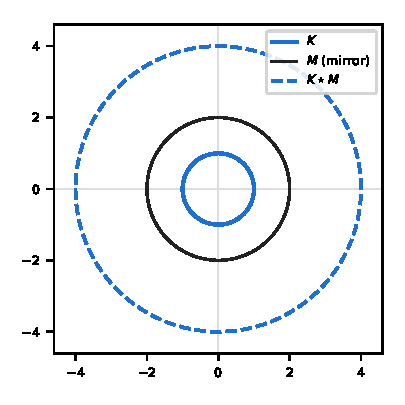
\includegraphics[width=0.31\textwidth]{examples16_figs/ex05.pdf}\\[-2pt]{\footnotesize Real picture: concentric, no finite common point.}\end{center}

\needspace{12\baselineskip}\subsection*{Example 6. Two lines at $60^\circ$}
\textbf{Exercise.} Reflect the $x$-axis in the line $y=\sqrt3\,x$. Compute $\kappa$ and the common points.

\smallskip\textbf{Solution.} \textbf{Inputs.} $L_1=[0:0:1:0]$, i.e.\ $y=0$; \ $L_2=[0:\sqrt{3}:-1:0]$, i.e.\ $y=\sqrt3\,x$. \textbf{Numbers.} $Q(L_1)=1$, $Q(L_2)=4$, $\langle L_1,L_2\rangle=-1$, $\kappa=\frac{1}{4}$. \textbf{Image.} $L_1\star L_2=L_1-\tfrac{2\langle L_1,L_2\rangle}{Q(L_2)}L_2\sim[0:1:\frac{\sqrt{3}}{3}:0]$, i.e.\ $x + \frac{\sqrt{3} y}{3}=0$. \textbf{Common points} (finite, of $L_1$ and $L_2$): $\left(0,\ 0\right)$ --- one finite point (and $\infty$). $\kappa=\tfrac14=\cos^2 60^\circ$. The image $y=-\sqrt3\,x$ makes $120^\circ$ with the $x$-axis. The finite common point is the origin; the second is $\infty=[0:0:0:1]$, shared by all lines ($a=0$).

\smallskip\emph{Why it is fun.} For two lines, $\kappa$ is literally $\cos^2$ of the angle (see Example 13 for what composing does).
\begin{center}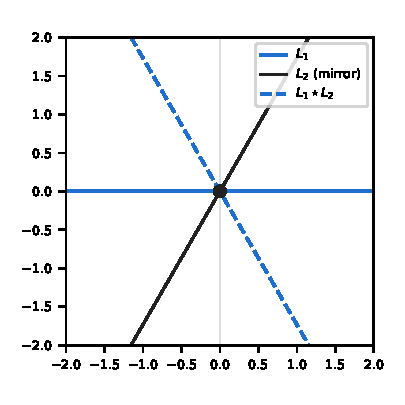
\includegraphics[width=0.31\textwidth]{examples16_figs/ex06.pdf}\\[-2pt]{\footnotesize Real picture: the image line is at $120^\circ$.}\end{center}

\needspace{12\baselineskip}\subsection*{Example 7. Invert a line: $x=2$ in the unit circle}
\textbf{Exercise.} Compute $L\star K$ for $L:\;x=2$ and compare with Example 2, where the roles were swapped.

\smallskip\textbf{Solution.} \textbf{Inputs.} $L=[0:1:0:-2]$, i.e.\ $x=2$; \ $K=[1:0:0:-1]$, i.e.\ $x^2+y^2=1$. \textbf{Numbers.} $Q(L)=1$, $Q(K)=4$, $\langle L,K\rangle=4$, $\kappa=4$. \textbf{Image.} $L\star K=L-\tfrac{2\langle L,K\rangle}{Q(K)}K\sim[1:- \frac{1}{2}:0:0]$, i.e.\ $x^{2} - \frac{x}{2} + y^{2}=0$. \textbf{Common points} (finite, of $L$ and $K$): $\left(2,\ - \sqrt{3} i\right)$, $\left(2,\ \sqrt{3} i\right)$ --- conjugate pair. $L\star K$ is the circle $x^2+y^2=\tfrac x2$, centre $(\tfrac14,0)$, radius $\tfrac14$, through the origin, which is the image of $\infty$. Like $K\star L$ in Example 2, it passes through the hidden points $(2,\pm i\sqrt3)$. The value $\kappa=4$ is the same, because $\kappa$ is symmetric.

\smallskip\emph{Why it is fun.} $\star$ is not commutative: $K\star L\neq L\star K$, yet both live in the pencil spanned by $K$ and $L$.
\begin{center}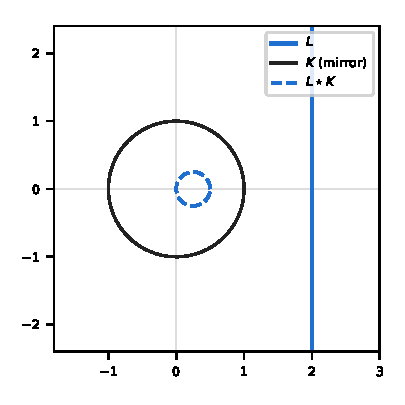
\includegraphics[width=0.31\textwidth]{examples16_figs/ex07.pdf}\\[-2pt]{\footnotesize Real picture: the common points $(2,\pm i\sqrt3)$ are not drawn.}\end{center}

\needspace{12\baselineskip}\subsection*{Example 8. A circle with complex centre: $(x-i)^2+y^2=1$}
\textbf{Exercise.} Let $C:\;(x-i)^2+y^2=1$. Reflect it in the $y$-axis. Then meet $C$ with the $x$-axis.

\smallskip\textbf{Solution.} \textbf{Inputs.} $C=[1:- 2 i:0:-2]$, i.e.\ $(x-i)^2+y^2=1$; \ $L=[0:1:0:0]$, i.e.\ $x=0$. \textbf{Numbers.} $Q(C)=4$, $Q(L)=1$, $\langle C,L\rangle=- 2 i$, $\kappa=-1$. \textbf{Image.} $C\star L=C-\tfrac{2\langle C,L\rangle}{Q(L)}L\sim[1:2 i:0:-2]$, i.e.\ $x^{2} + 2 i x + y^{2} - 2=0$. \textbf{Common points} (finite, of $C$ and $L$): $\left(0,\ - \sqrt{2}\right)$, $\left(0,\ \sqrt{2}\right)$ --- two real. $Q(C)=4$, a ``radius'' of $1$. $\kappa=-1<0$, which is impossible for a real circle and a real line. The reflection moves the centre from $i$ to $-i$: $C\star L$ is $(x+i)^2+y^2=1$. With the $y$-axis $C$ meets in the real points $(0,\pm\sqrt2)$; these are the whole real trace of $C$, where $\mathrm{Re}=x^2+y^2-2$ and $\mathrm{Im}=-2x$ vanish together. With the $x$-axis $M'=[0:0:1:0]$: $\langle C,M'\rangle=0$, so $C\star M'=C$, and the common points are $(1+i,0)$ and $(-1+i,0)$, complex and \emph{not} conjugate.

\smallskip\emph{Why it is fun.} A complex circle can cross a real line in two real points, and in non-conjugate complex points.
\begin{center}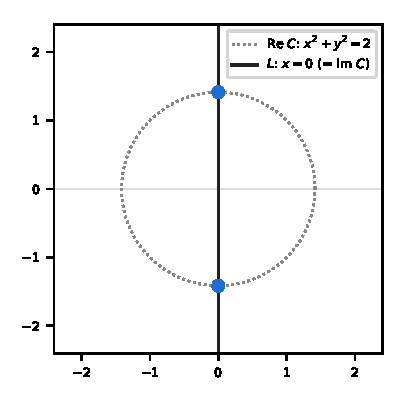
\includegraphics[width=0.31\textwidth]{examples16_figs/ex08.pdf}\\[-2pt]{\footnotesize Only the real trace of $C$ is drawn: $\mathrm{Re}\,C$ (grey circle) and $\mathrm{Im}\,C$ (the line $x=0$, which is also the mirror) meet at $(0,\pm\sqrt2)$.}\end{center}

\needspace{12\baselineskip}\subsection*{Example 9. The circle of imaginary radius $x^2+y^2=-1$}
\textbf{Exercise.} $S:\;x^2+y^2=-1$ has no real points. Use it as a mirror for $D:\;(x-1)^2+y^2=1$, and show $K\star S=K$ for the unit circle.

\smallskip\textbf{Solution.} \textbf{Inputs.} $D=[1:-2:0:0]$, i.e.\ $(x-1)^2+y^2=1$; \ $S=[1:0:0:1]$, i.e.\ $x^2+y^2=-1$. \textbf{Numbers.} $Q(D)=4$, $Q(S)=-4$, $\langle D,S\rangle=-2$, $\kappa=- \frac{1}{4}$. \textbf{Image.} $D\star S=D-\tfrac{2\langle D,S\rangle}{Q(S)}S\sim[0:1:0:\frac{1}{2}]$, i.e.\ $x + \frac{1}{2}=0$. \textbf{Common points} (finite, of $D$ and $S$): $\left(- \frac{1}{2},\ - \frac{\sqrt{5} i}{2}\right)$, $\left(- \frac{1}{2},\ \frac{\sqrt{5} i}{2}\right)$ --- conjugate pair. $Q(S)=-4<0$. $D\star S$ is the real line $x=-\tfrac12$. In general, reflection in $S$ sends the point $p$ to $-p/|p|^2$ (inversion composed with the half-turn), a real map with no real fixed points. $\langle K,S\rangle=0$, so $K\star S=K$: the unit circle is ``orthogonal'' to $S$ (the map swaps antipodes of $K$). $D$ and $S$ meet in the conjugate pair $(-\tfrac12,\pm\tfrac{\sqrt5}2i)$.

\smallskip\emph{Why it is fun.} An invisible mirror acts visibly: it maps real circles to real circles, and $\kappa=-\tfrac14<0$ betrays it.
\begin{center}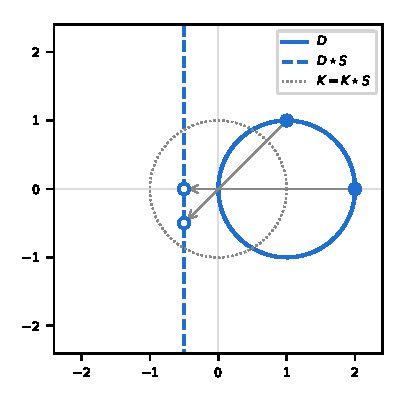
\includegraphics[width=0.31\textwidth]{examples16_figs/ex09.pdf}\\[-2pt]{\footnotesize $S$ has no real points (not drawn). Reflection in $S$ is $p\mapsto-p/|p|^2$: $D$ goes to the line $x=-\tfrac12$.}\end{center}

\needspace{12\baselineskip}\subsection*{Example 10. Isotropic lines: $y=ix$, $y=ix+1$, and $y=2ix$}
\textbf{Exercise.} Which of $y=ix$, $y=ix+1$, $y=2ix$ can be a mirror? Meet each with $K$.

\smallskip\textbf{Solution.} \textbf{Inputs.} $K=[1:0:0:-1]$, i.e.\ $x^2+y^2=1$; \ $L=[0:2 i:-1:0]$, i.e.\ $y=2ix$. \textbf{Numbers.} $Q(K)=4$, $Q(L)=-3$, $\langle K,L\rangle=0$, $\kappa=0$. \textbf{Image.} $K\star L=K-\tfrac{2\langle K,L\rangle}{Q(L)}L\sim[1:0:0:-1]$, i.e.\ $x^{2} + y^{2} - 1=0$. \textbf{Common points} (finite, of $K$ and $L$): $\left(- \frac{\sqrt{3} i}{3},\ \frac{2 \sqrt{3}}{3}\right)$, $\left(\frac{\sqrt{3} i}{3},\ - \frac{2 \sqrt{3}}{3}\right)$ --- two complex, not conjugate. $y=ix$ is $[0:i:-1:0]\sim[0:1:i:0]$ and $y=ix+1$ is $[0:i:-1:1]$; both have $Q=i^2+(-1)^2=0$, so neither can be a mirror. On $y=ix$ we have $x^2+y^2\equiv0$, so $K$ gives $-1=0$: no finite point. On the Möbius quadric the line $[0:1:i:0]$ is \emph{itself} a null vector with $\langle K,\cdot\rangle=0$, the double common point (tangency ``at $\infty$''). $y=ix+1$ meets $K$ in the single finite point $(0,1)$, which is also its only real point; the other common point is again $[0:1:i:0]$. $y=2ix$ has $Q=-3\neq0$: a fine mirror. It passes through the centre, so $\langle K,L\rangle=0$ and $K\star L=K$, with common points $\pm(\tfrac{i}{\sqrt3},-\tfrac{2}{\sqrt3})$: each has one real and one imaginary coordinate, and they are not conjugate.

\smallskip\emph{Why it is fun.} Only the slopes $\pm i$ are forbidden. With them the ``always two finite points'' rule drops to one or zero.
\begin{center}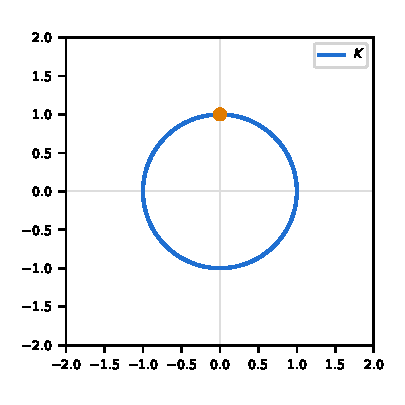
\includegraphics[width=0.31\textwidth]{examples16_figs/ex10.pdf}\\[-2pt]{\footnotesize The non-real line $y=ix+1$ has one real point, $(0,1)$, which is also its only finite common point with $K$.}\end{center}

\needspace{12\baselineskip}\subsection*{Example 11. A point as input: the point-circle at $(1,1)$}
\textbf{Exercise.} Treat the point $(1,1)$ as the circle $P$ of radius $0$. Compute $P\star K$. What are $\kappa$ and $P\cap K$?

\smallskip\textbf{Solution.} \textbf{Inputs.} $P=[1:-2:-2:2]$, i.e.\ $(x-1)^2+(y-1)^2=0$; \ $K=[1:0:0:-1]$, i.e.\ $x^2+y^2=1$. \textbf{Numbers.} $Q(P)=0$, $Q(K)=4$, $\langle P,K\rangle=-2$, $\kappa=\text{undefined } (Q(\cdot)=0)$. \textbf{Image.} $P\star K=P-\tfrac{2\langle P,K\rangle}{Q(K)}K\sim[1:-1:-1:\frac{1}{2}]$, i.e.\ $x^{2} - x + y^{2} - y + \frac{1}{2}=0$. \textbf{Common points} (finite, of $P$ and $K$): $\left(\frac{3}{4} - \frac{i}{4},\ \frac{3}{4} + \frac{i}{4}\right)$, $\left(\frac{3}{4} + \frac{i}{4},\ \frac{3}{4} - \frac{i}{4}\right)$ --- conjugate pair. $Q(P)=0$, so $P\star K$ is again a point-circle (since $Q$ is preserved): the point $(\tfrac12,\tfrac12)$, the classical inverse of $(1,1)$. $K\star P$ is undefined and $\kappa$ is undefined ($Q(P)Q(K)=0$); only $\langle P,K\rangle=-2K(1,1)=-2$, minus twice the power, is meaningful. $P$ is the pair of isotropic lines through $(1,1)$, and it meets $K$ in the conjugate pair $(\tfrac34\mp\tfrac i4,\tfrac34\pm\tfrac i4)$: the two points of $K$ at zero (complex) distance from $(1,1)$.

\smallskip\emph{Why it is fun.} Points are circles of $Q=0$: inputs yes, mirrors no.
\begin{center}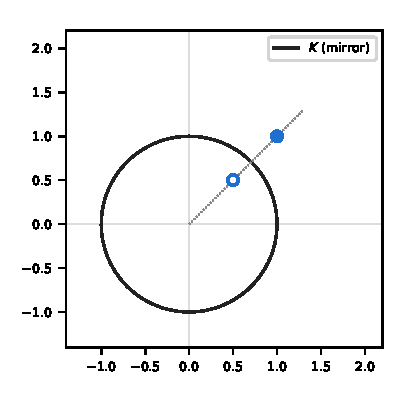
\includegraphics[width=0.31\textwidth]{examples16_figs/ex11.pdf}\\[-2pt]{\footnotesize Real picture: the point $(1,1)$ and its inverse $(\tfrac12,\tfrac12)$; the common points are complex.}\end{center}

\needspace{12\baselineskip}\subsection*{Example 12. A complex mirror makes a real circle non-real}
\textbf{Exercise.} Reflect the real unit circle in $M:\;(x-i)^2+y^2=1$. Is the image real? Where is it real?

\smallskip\textbf{Solution.} \textbf{Inputs.} $K=[1:0:0:-1]$, i.e.\ $x^2+y^2=1$; \ $M=[1:- 2 i:0:-2]$, i.e.\ $(x-i)^2+y^2=1$. \textbf{Numbers.} $Q(K)=4$, $Q(M)=4$, $\langle K,M\rangle=6$, $\kappa=\frac{9}{4}$. \textbf{Image.} $K\star M=K-\tfrac{2\langle K,M\rangle}{Q(M)}M\sim[1:- 3 i:0:- \frac{5}{2}]$, i.e.\ $x^{2} - 3 i x + y^{2} - \frac{5}{2}=0$. \textbf{Common points} (finite, of $K$ and $M$): $\left(\frac{i}{2},\ - \frac{\sqrt{5}}{2}\right)$, $\left(\frac{i}{2},\ \frac{\sqrt{5}}{2}\right)$ --- two complex, not conjugate. $K\star M$ is $x^2+y^2-3ix-\tfrac52=0$, i.e.\ $(x-\tfrac{3i}2)^2+y^2=\tfrac14$: complex centre, ``radius'' $\tfrac12$. Its real trace ($x=0$ and $x^2+y^2=\tfrac52$) is the two points $(0,\pm\sqrt{5/2})$. $K$ and $M$ meet at $(\tfrac i2,\pm\tfrac{\sqrt5}2)$: mixed, with imaginary $x$ and real $y$.

\smallskip\emph{Why it is fun.} Realness is not preserved: a complex reflection takes a real circle off the real plane, leaving just two real points behind.
\begin{center}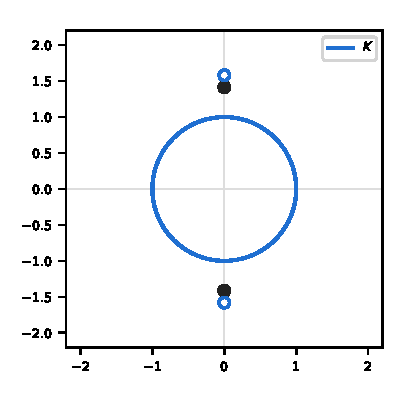
\includegraphics[width=0.31\textwidth]{examples16_figs/ex12.pdf}\\[-2pt]{\footnotesize Real picture: $K$, plus the real traces of $M$ (dots $(0,\pm\sqrt2)$) and of $K\star M$ (rings $(0,\pm\sqrt{5/2})$).}\end{center}

\needspace{12\baselineskip}\subsection*{Example 13. Two mirrors make a rotation of order 2, 3, 4, $\infty$, or a complex angle}
\textbf{Exercise.} For lines through $0$ at angle $\theta$, $s_{L_2}\circ s_{L_1}$ is a rotation by $2\theta$. Tabulate $\kappa$ and the order for $\theta=90^\circ,60^\circ,45^\circ$ and for parallel lines. Then take $L_2:\;y=\tfrac{\sqrt3}{2}i\,x$.

\smallskip\textbf{Solution.} \textbf{Inputs.} $L_1=[0:0:1:0]$, i.e.\ $y=0$; \ $L_2=[0:\frac{\sqrt{3} i}{2}:-1:0]$, i.e.\ $y=\tfrac{\sqrt3}{2}i\,x$. \textbf{Numbers.} $Q(L_1)=1$, $Q(L_2)=\frac{1}{4}$, $\langle L_1,L_2\rangle=-1$, $\kappa=4$. \textbf{Image.} $L_1\star L_2=L_1-\tfrac{2\langle L_1,L_2\rangle}{Q(L_2)}L_2\sim[0:1:\frac{7 \sqrt{3} i}{12}:0]$, i.e.\ $x + \frac{7 \sqrt{3} i y}{12}=0$. \textbf{Common points} (finite, of $L_1$ and $L_2$): $\left(0,\ 0\right)$ --- one finite point (and $\infty$). Real cases: $\theta=90^\circ$ gives $\kappa=0$ and a half-turn (order $2$); $60^\circ$ gives $\kappa=\tfrac14$ (order $3$); $45^\circ$ gives $\kappa=\tfrac12$ (order $4$). The parallel lines $x=0$, $x=1$ give $\kappa=1$ (tangent at $\infty$) and the translation by $2$ (infinite order). The 4×4 matrices satisfy $(R_2R_1)^n=I$ for $n=2,3,4$. Complex case: $\kappa=4$, so ``$\cos\theta=2$''. In isotropic coordinates $u=x+iy$, $v=x-iy$ the composition is $u\mapsto\lambda u$, $v\mapsto v/\lambda$ with $\lambda=(2+\sqrt3)^{\pm2}=7\mp4\sqrt3$: a boost, of infinite order. It sends real points (where $v=\bar u$) to non-real ones. $L_1\star L_2$ is the line $x+\tfrac{7\sqrt3}{12}i\,y=0$, whose slope $\tfrac{4\sqrt3}{7}i=\tan2\theta$.

\smallskip\emph{Why it is fun.} $\kappa=\cos^2\theta$ keeps working when the angle is complex, and a rotation turns into a squeeze.
\begin{center}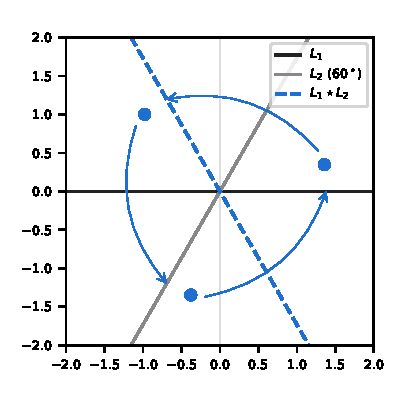
\includegraphics[width=0.31\textwidth]{examples16_figs/ex13.pdf}\\[-2pt]{\footnotesize Real case $60^\circ$: $s_{L_2}\circ s_{L_1}$ rotates by $120^\circ$ (order 3). The complex case has no real picture.}\end{center}

\needspace{12\baselineskip}\subsection*{Example 14. The kei law, checked by hand}
\textbf{Exercise.} With $A=K$, $B:\;x=\tfrac12$, $L:\;x+2y=2$, verify $A\star A\sim A$, $(A\star L)\star L=A$, and $(A\star B)\star L=(A\star L)\star(B\star L)$. Is $\star$ associative?

\smallskip\textbf{Solution.} \textbf{Inputs.} $A=[1:0:0:-1]$, i.e.\ $x^2+y^2=1$; \ $L=[0:1:2:-2]$, i.e.\ $x+2y=2$. \textbf{Numbers.} $Q(A)=4$, $Q(L)=5$, $\langle A,L\rangle=4$, $\kappa=\frac{4}{5}$. \textbf{Image.} $A\star L=A-\tfrac{2\langle A,L\rangle}{Q(L)}L\sim[1:- \frac{8}{5}:- \frac{16}{5}:\frac{11}{5}]$, i.e.\ $x^{2} - \frac{8 x}{5} + y^{2} - \frac{16 y}{5} + \frac{11}{5}=0$. \textbf{Common points} (finite, of $A$ and $L$): $\left(0,\ 1\right)$, $\left(\frac{4}{5},\ \frac{3}{5}\right)$ --- two real. $A\star A=-A\sim A$. $A\star B\sim[1:-2:0:0]$, $A\star L\sim[1:- \frac{8}{5}:- \frac{16}{5}:\frac{11}{5}]$, $B\star L\sim[0:1:- \frac{4}{3}:\frac{1}{2}]$. Then $(A\star B)\star L\sim[1:- \frac{14}{5}:- \frac{8}{5}:\frac{8}{5}]$ and $(A\star L)\star(B\star L)\sim[1:- \frac{14}{5}:- \frac{8}{5}:\frac{8}{5}]$: equal, which is the kei law. But $A\star(B\star L)\sim[1:\frac{18}{25}:- \frac{24}{25}:- \frac{16}{25}]$, so $\star$ is not associative. Applying $L$ twice returns $A$.

\smallskip\emph{Why it is fun.} The three kei axioms come from the fact that reflection is an isometry of $\langle\,,\rangle$; associativity fails.
\begin{center}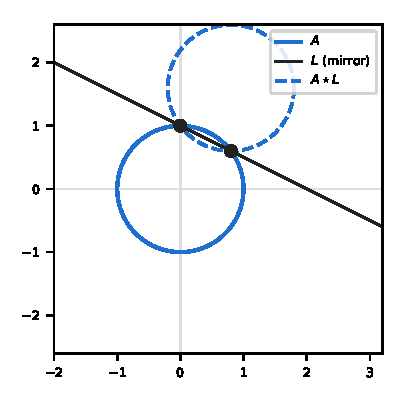
\includegraphics[width=0.31\textwidth]{examples16_figs/ex14.pdf}\\[-2pt]{\footnotesize Real picture of $A$, $L$, $A\star L$.}\end{center}

\needspace{12\baselineskip}\subsection*{Example 15. Tangency with complex coefficients}
\textbf{Exercise.} Find $c$ so that $y=2ix+c$ is tangent to $K$, then compute the double point and $K\star L$.

\smallskip\textbf{Solution.} \textbf{Inputs.} $K=[1:0:0:-1]$, i.e.\ $x^2+y^2=1$; \ $L=[0:2 i:-1:\sqrt{3} i]$, i.e.\ $y=2ix+i\sqrt3$. \textbf{Numbers.} $Q(K)=4$, $Q(L)=-3$, $\langle K,L\rangle=- 2 \sqrt{3} i$, $\kappa=1$. \textbf{Image.} $K\star L=K-\tfrac{2\langle K,L\rangle}{Q(L)}L\sim[1:\frac{8 \sqrt{3}}{3}:\frac{4 \sqrt{3} i}{3}:3]$, i.e.\ $x^{2} + \frac{8 \sqrt{3} x}{3} + y^{2} + \frac{4 \sqrt{3} i y}{3} + 3=0$. \textbf{Common points} (finite, of $K$ and $L$): $\left(- \frac{2 \sqrt{3}}{3},\ - \frac{\sqrt{3} i}{3}\right)$ --- one double point (complex). A line $y=mx+c$ is tangent to $K$ iff $c^2=1+m^2$, which is $\kappa=1$. For $m=2i$ this gives $c^2=-3$, so $c=i\sqrt3$. The double point is $(-\tfrac2{\sqrt3},-\tfrac{i}{\sqrt3})$. The image $K\star L$ is tangent to $K$ there too: $\kappa(K\star L,L)=\kappa(K,L)=1$, by invariance under $s_L$, which fixes $L$.

\smallskip\emph{Why it is fun.} ``Touching'' needs no picture: a complex line is tangent to the real unit circle at a point with an imaginary $y$.
{\footnotesize (No real picture: every point involved is non-real.)}

\needspace{12\baselineskip}\subsection*{Example 16. Find the mirror: swap two disjoint circles}
\textbf{Exercise.} Find all mirrors $M$ with $K\star M=C_2$ for $C_2:\;(x-4)^2+y^2=4$.

\smallskip\textbf{Solution.} \textbf{Inputs.} $K=[1:0:0:-1]$, i.e.\ $x^2+y^2=1$; \ $C_2=[\frac{1}{2}:-4:0:6]$, i.e.\ $(x-4)^2+y^2=4$. \textbf{Numbers.} $Q(K)=4$, $Q(C_2)=4$, $\langle K,C_2\rangle=-11$, $\kappa=\frac{121}{16}$. \textbf{Image.} $K\star C_2=K-\tfrac{2\langle K,C_2\rangle}{Q(C_2)}C_2\sim[1:- \frac{88}{15}:0:\frac{128}{15}]$, i.e.\ $x^{2} - \frac{88 x}{15} + y^{2} + \frac{128}{15}=0$. \textbf{Common points} (finite, of $K$ and $C_2$): $\left(\frac{13}{8},\ - \frac{\sqrt{105} i}{8}\right)$, $\left(\frac{13}{8},\ \frac{\sqrt{105} i}{8}\right)$ --- conjugate pair. Rescale $C_2$ to $C_2'=[\tfrac12:-4:0:6]$ so that $Q(C_2')=Q(K)=4$ (always possible over $\mathbb C$). If $Q(C)=Q(C')$, then $M=C-C'$ gives $\langle C,M\rangle=Q(C)-\langle C,C'\rangle=\tfrac12Q(M)$, so $C\star M=C'$; the same works for $M=C+C'$, since $-C'\sim C'$. Here $M_-=K-C_2'\sim[1:8:0:-14]$, the real circle $(x+4)^2+y^2=30$, and $M_+=K+C_2'\sim[1:-\tfrac83:0:\tfrac{10}3]$, i.e.\ $(x-\tfrac43)^2+y^2=-\tfrac{14}9$, a circle of \emph{imaginary radius}. There are no others: $K\star M=K-kM$ forces $M$ into the pencil $K-\lambda C_2'$, and there only $\lambda=\pm1$ works. They are orthogonal, $\langle M_-,M_+\rangle=0$, and both pass through the hidden points $(\tfrac{13}8,\pm\tfrac{\sqrt{105}}8 i)$. For the tangent pair $(x-3)^2+y^2=4$, $M_+$ degenerates to the point-circle at the contact point $(1,0)$. (The ``Image'' line above is $K\star C_2$, for comparison only.)

\smallskip\emph{Why it is fun.} Two disjoint circles have two swapping mirrors, one real and one of imaginary radius; when they touch, the second degenerates to a point.
\begin{center}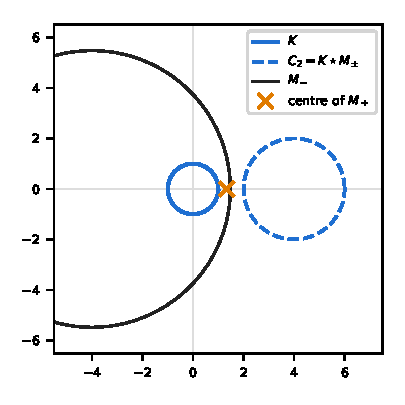
\includegraphics[width=0.31\textwidth]{examples16_figs/ex16.pdf}\\[-2pt]{\footnotesize Real picture: $K$, $C_2$ and the real mirror $M_-$. The imaginary mirror $M_+$ (centre $\times$) has no real points.}\end{center}

\end{document}